\documentclass[10pt]{article}
\usepackage[utf8]{inputenc}
\usepackage[T1]{fontenc}
\usepackage{amsmath}
\usepackage{amsfonts}
\usepackage{amssymb}
\usepackage{stmaryrd}
\usepackage{hyperref}
\hypersetup{colorlinks=true, linkcolor=blue, filecolor=magenta, urlcolor=cyan,}
\urlstyle{same}
\usepackage{graphicx}
\usepackage[export]{adjustbox}
\usepackage{mdframed}
\usepackage{booktabs,array,multirow}
\usepackage{esint}
\usepackage{xeCJK}
\usepackage{adjustbox}
\newcommand{\HRule}{\begin{center}\rule{0.5\linewidth}{0.2mm}\end{center}}
\graphicspath{ {./images/} }
\begin{document}



\section*{2. 两个电极}

\section*{3. 流向}

电子流向:\_\_\_

电流流向: 阴一阳

\text{\textbackslash} x离子流向:异性相吸(阳离子→阴极)

【经典】某同学为了使反应 \(2\mathrm{{HC}}1 + 2\mathrm{{Ag}} = 2\mathrm{{AgC}}1 + {\mathrm{H}}_{2} \uparrow\) 能进行,设计了如图所示的四个实验,你认为可行的方案是 ( ) B. C. D.

\begin{center}
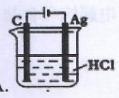
\includegraphics[max width=0.2\textwidth]{images/0190d9a9-6e54-7ef1-97c3-2701896ca5e8_0_699548.jpg}
\end{center}

\begin{center}
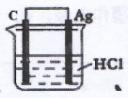
\includegraphics[max width=0.2\textwidth]{images/0190d9a9-6e54-7ef1-97c3-2701896ca5e8_0_942435.jpg}
\end{center}

\begin{center}
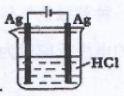
\includegraphics[max width=0.2\textwidth]{images/0190d9a9-6e54-7ef1-97c3-2701896ca5e8_0_433745.jpg}
\end{center}

\begin{center}
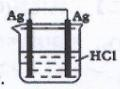
\includegraphics[max width=0.2\textwidth]{images/0190d9a9-6e54-7ef1-97c3-2701896ca5e8_0_668314.jpg}
\end{center}

\end{document}